% Created by tikzDevice version 0.6.2-92-0ad2792 on 2013-01-11 06:31:19
% !TEX encoding = UTF-8 Unicode
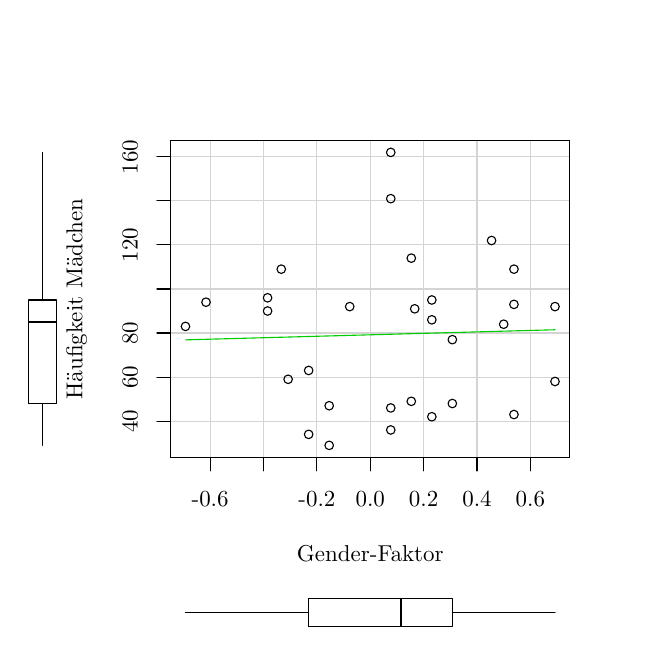
\begin{tikzpicture}[x=1pt,y=1pt]
\definecolor[named]{fillColor}{rgb}{1.00,1.00,1.00}
\path[use as bounding box,fill=fillColor,fill opacity=0.00] (0,0) rectangle (216.81,216.81);
\begin{scope}
\path[clip] (  0.00, 61.64) rectangle ( 10.84,175.97);
\definecolor[named]{drawColor}{rgb}{0.00,0.00,0.00}

\path[draw=drawColor,line width= 0.4pt,line join=round,line cap=round] (  0.40, 81.00) --
	( 10.44, 81.00) --
	( 10.44,118.41) --
	(  0.40,118.41) --
	(  0.40, 81.00);

\path[draw=drawColor,line width= 0.4pt,line join=round,line cap=round] (  0.40,110.45) --
	( 10.44,110.45);

\path[draw=drawColor,line width= 0.4pt,line join=round,line cap=round] (  5.42, 65.87) --
	(  5.42, 81.00);

\path[draw=drawColor,line width= 0.4pt,line join=round,line cap=round] (  5.42,118.41) --
	(  5.42,171.74);
\end{scope}
\begin{scope}
\path[clip] ( 51.68,  0.00) rectangle (195.89, 10.84);
\definecolor[named]{drawColor}{rgb}{0.00,0.00,0.00}

\path[draw=drawColor,line width= 0.4pt,line join=round,line cap=round] (101.53,  0.40) --
	(101.53, 10.44) --
	(153.46, 10.44) --
	(153.46,  0.40) --
	(101.53,  0.40);

\path[draw=drawColor,line width= 0.4pt,line join=round,line cap=round] (134.91,  0.40) --
	(134.91, 10.44);

\path[draw=drawColor,line width= 0.4pt,line join=round,line cap=round] ( 57.02,  5.42) --
	(101.53,  5.42);

\path[draw=drawColor,line width= 0.4pt,line join=round,line cap=round] (153.46,  5.42) --
	(190.55,  5.42);
\end{scope}
\begin{scope}
\path[clip] (  0.00,  0.00) rectangle (216.81,216.81);
\definecolor[named]{drawColor}{rgb}{0.00,0.00,0.00}

\path[draw=drawColor,line width= 0.4pt,line join=round,line cap=round] ( 65.92, 61.64) -- (181.65, 61.64);

\path[draw=drawColor,line width= 0.4pt,line join=round,line cap=round] ( 65.92, 61.64) -- ( 65.92, 56.66);

\path[draw=drawColor,line width= 0.4pt,line join=round,line cap=round] ( 85.21, 61.64) -- ( 85.21, 56.66);

\path[draw=drawColor,line width= 0.4pt,line join=round,line cap=round] (104.50, 61.64) -- (104.50, 56.66);

\path[draw=drawColor,line width= 0.4pt,line join=round,line cap=round] (123.79, 61.64) -- (123.79, 56.66);

\path[draw=drawColor,line width= 0.4pt,line join=round,line cap=round] (143.07, 61.64) -- (143.07, 56.66);

\path[draw=drawColor,line width= 0.4pt,line join=round,line cap=round] (162.36, 61.64) -- (162.36, 56.66);

\path[draw=drawColor,line width= 0.4pt,line join=round,line cap=round] (181.65, 61.64) -- (181.65, 56.66);

\node[text=drawColor,anchor=base,inner sep=0pt, outer sep=0pt, scale=  0.83] at ( 65.92, 43.71) {-0.6};

\node[text=drawColor,anchor=base,inner sep=0pt, outer sep=0pt, scale=  0.83] at (104.50, 43.71) {-0.2};

\node[text=drawColor,anchor=base,inner sep=0pt, outer sep=0pt, scale=  0.83] at (123.79, 43.71) {0.0};

\node[text=drawColor,anchor=base,inner sep=0pt, outer sep=0pt, scale=  0.83] at (143.07, 43.71) {0.2};

\node[text=drawColor,anchor=base,inner sep=0pt, outer sep=0pt, scale=  0.83] at (162.36, 43.71) {0.4};

\node[text=drawColor,anchor=base,inner sep=0pt, outer sep=0pt, scale=  0.83] at (181.65, 43.71) {0.6};

\path[draw=drawColor,line width= 0.4pt,line join=round,line cap=round] ( 51.68, 74.63) -- ( 51.68,170.15);

\path[draw=drawColor,line width= 0.4pt,line join=round,line cap=round] ( 51.68, 74.63) -- ( 46.70, 74.63);

\path[draw=drawColor,line width= 0.4pt,line join=round,line cap=round] ( 51.68, 90.55) -- ( 46.70, 90.55);

\path[draw=drawColor,line width= 0.4pt,line join=round,line cap=round] ( 51.68,106.47) -- ( 46.70,106.47);

\path[draw=drawColor,line width= 0.4pt,line join=round,line cap=round] ( 51.68,122.39) -- ( 46.70,122.39);

\path[draw=drawColor,line width= 0.4pt,line join=round,line cap=round] ( 51.68,138.31) -- ( 46.70,138.31);

\path[draw=drawColor,line width= 0.4pt,line join=round,line cap=round] ( 51.68,154.23) -- ( 46.70,154.23);

\path[draw=drawColor,line width= 0.4pt,line join=round,line cap=round] ( 51.68,170.15) -- ( 46.70,170.15);

\node[text=drawColor,rotate= 90.00,anchor=base,inner sep=0pt, outer sep=0pt, scale=  0.83] at ( 39.72, 74.63) {40};

\node[text=drawColor,rotate= 90.00,anchor=base,inner sep=0pt, outer sep=0pt, scale=  0.83] at ( 39.72, 90.55) {60};

\node[text=drawColor,rotate= 90.00,anchor=base,inner sep=0pt, outer sep=0pt, scale=  0.83] at ( 39.72,106.47) {80};

\node[text=drawColor,rotate= 90.00,anchor=base,inner sep=0pt, outer sep=0pt, scale=  0.83] at ( 39.72,138.31) {120};

\node[text=drawColor,rotate= 90.00,anchor=base,inner sep=0pt, outer sep=0pt, scale=  0.83] at ( 39.72,170.15) {160};

\path[draw=drawColor,line width= 0.4pt,line join=round,line cap=round] ( 51.68, 61.64) --
	(195.89, 61.64) --
	(195.89,175.97) --
	( 51.68,175.97) --
	( 51.68, 61.64);
\end{scope}
\begin{scope}
\path[clip] ( 10.84, 10.84) rectangle (216.81,216.81);
\definecolor[named]{drawColor}{rgb}{0.00,0.00,0.00}

\node[text=drawColor,anchor=base,inner sep=0pt, outer sep=0pt, scale=  0.83] at (123.79, 23.79) {Gender-Faktor};

\node[text=drawColor,rotate= 90.00,anchor=base,inner sep=0pt, outer sep=0pt, scale=  0.83] at ( 19.80,118.81) {Häufigkeit Mädchen};
\end{scope}
\begin{scope}
\path[clip] ( 51.68, 61.64) rectangle (195.89,175.97);
\definecolor[named]{drawColor}{rgb}{0.83,0.83,0.83}

\path[draw=drawColor,line width= 0.4pt,line join=round,line cap=round] ( 65.92, 61.64) -- ( 65.92,175.97);

\path[draw=drawColor,line width= 0.4pt,line join=round,line cap=round] ( 85.21, 61.64) -- ( 85.21,175.97);

\path[draw=drawColor,line width= 0.4pt,line join=round,line cap=round] (104.50, 61.64) -- (104.50,175.97);

\path[draw=drawColor,line width= 0.4pt,line join=round,line cap=round] (123.79, 61.64) -- (123.79,175.97);

\path[draw=drawColor,line width= 0.4pt,line join=round,line cap=round] (143.07, 61.64) -- (143.07,175.97);

\path[draw=drawColor,line width= 0.4pt,line join=round,line cap=round] (162.36, 61.64) -- (162.36,175.97);

\path[draw=drawColor,line width= 0.4pt,line join=round,line cap=round] (181.65, 61.64) -- (181.65,175.97);

\path[draw=drawColor,line width= 0.4pt,line join=round,line cap=round] ( 51.68, 74.63) -- (195.89, 74.63);

\path[draw=drawColor,line width= 0.4pt,line join=round,line cap=round] ( 51.68, 90.55) -- (195.89, 90.55);

\path[draw=drawColor,line width= 0.4pt,line join=round,line cap=round] ( 51.68,106.47) -- (195.89,106.47);

\path[draw=drawColor,line width= 0.4pt,line join=round,line cap=round] ( 51.68,122.39) -- (195.89,122.39);

\path[draw=drawColor,line width= 0.4pt,line join=round,line cap=round] ( 51.68,138.31) -- (195.89,138.31);

\path[draw=drawColor,line width= 0.4pt,line join=round,line cap=round] ( 51.68,154.23) -- (195.89,154.23);

\path[draw=drawColor,line width= 0.4pt,line join=round,line cap=round] ( 51.68,170.15) -- (195.89,170.15);
\end{scope}
\begin{scope}
\path[clip] (  0.00,  0.00) rectangle (216.81,216.81);
\definecolor[named]{drawColor}{rgb}{0.00,0.00,0.00}

\path[draw=drawColor,line width= 0.4pt,line join=round,line cap=round] ( 51.68, 61.64) --
	(195.89, 61.64) --
	(195.89,175.97) --
	( 51.68,175.97) --
	( 51.68, 61.64);
\end{scope}
\begin{scope}
\path[clip] ( 51.68, 61.64) rectangle (195.89,175.97);
\definecolor[named]{drawColor}{rgb}{0.00,0.00,0.00}

\path[draw=drawColor,line width= 0.4pt,line join=round,line cap=round] (131.20, 79.40) circle (  1.55);

\path[draw=drawColor,line width= 0.4pt,line join=round,line cap=round] (108.95, 65.87) circle (  1.55);

\path[draw=drawColor,line width= 0.4pt,line join=round,line cap=round] (108.95, 80.20) circle (  1.55);

\path[draw=drawColor,line width= 0.4pt,line join=round,line cap=round] (138.62,133.53) circle (  1.55);

\path[draw=drawColor,line width= 0.4pt,line join=round,line cap=round] (138.62, 81.79) circle (  1.55);

\path[draw=drawColor,line width= 0.4pt,line join=round,line cap=round] (153.46, 81.00) circle (  1.55);

\path[draw=drawColor,line width= 0.4pt,line join=round,line cap=round] (172.01,109.65) circle (  1.55);

\path[draw=drawColor,line width= 0.4pt,line join=round,line cap=round] ( 91.64,129.55) circle (  1.55);

\path[draw=drawColor,line width= 0.4pt,line join=round,line cap=round] (131.20,171.74) circle (  1.55);

\path[draw=drawColor,line width= 0.4pt,line join=round,line cap=round] ( 64.44,117.61) circle (  1.55);

\path[draw=drawColor,line width= 0.4pt,line join=round,line cap=round] (131.20,155.02) circle (  1.55);

\path[draw=drawColor,line width= 0.4pt,line join=round,line cap=round] ( 94.11, 89.75) circle (  1.55);

\path[draw=drawColor,line width= 0.4pt,line join=round,line cap=round] (153.46,104.08) circle (  1.55);

\path[draw=drawColor,line width= 0.4pt,line join=round,line cap=round] (175.72,129.55) circle (  1.55);

\path[draw=drawColor,line width= 0.4pt,line join=round,line cap=round] (139.86,115.22) circle (  1.55);

\path[draw=drawColor,line width= 0.4pt,line join=round,line cap=round] (101.53, 69.85) circle (  1.55);

\path[draw=drawColor,line width= 0.4pt,line join=round,line cap=round] (131.20, 71.44) circle (  1.55);

\path[draw=drawColor,line width= 0.4pt,line join=round,line cap=round] (116.37,116.02) circle (  1.55);

\path[draw=drawColor,line width= 0.4pt,line join=round,line cap=round] (146.04, 76.22) circle (  1.55);

\path[draw=drawColor,line width= 0.4pt,line join=round,line cap=round] ( 86.69,119.20) circle (  1.55);

\path[draw=drawColor,line width= 0.4pt,line join=round,line cap=round] (190.55,116.02) circle (  1.55);

\path[draw=drawColor,line width= 0.4pt,line join=round,line cap=round] ( 86.69,114.43) circle (  1.55);

\path[draw=drawColor,line width= 0.4pt,line join=round,line cap=round] (175.72, 77.02) circle (  1.55);

\path[draw=drawColor,line width= 0.4pt,line join=round,line cap=round] ( 57.02,108.86) circle (  1.55);

\path[draw=drawColor,line width= 0.4pt,line join=round,line cap=round] (146.04,118.41) circle (  1.55);

\path[draw=drawColor,line width= 0.4pt,line join=round,line cap=round] (175.72,116.82) circle (  1.55);

\path[draw=drawColor,line width= 0.4pt,line join=round,line cap=round] (146.04,111.24) circle (  1.55);

\path[draw=drawColor,line width= 0.4pt,line join=round,line cap=round] (190.55, 88.96) circle (  1.55);

\path[draw=drawColor,line width= 0.4pt,line join=round,line cap=round] (167.62,139.90) circle (  1.55);

\path[draw=drawColor,line width= 0.4pt,line join=round,line cap=round] (101.53, 92.94) circle (  1.55);
\definecolor[named]{drawColor}{rgb}{0.00,0.80,0.00}

\path[draw=drawColor,line width= 0.4pt,line join=round,line cap=round] ( 57.02,104.00) --
	(190.55,107.65);
\end{scope}
\end{tikzpicture}
